\chapter{Introduction}
This project is about machine learning of different statistical classifiers.
Machine learning is about construct and study systems that can learn from data.
This could be used to train a system to recognize patterns in, for instance, emails and learn how to distinguish between spam and non-spam messages. In this project the classifiers are applied to reviews and the task is to categorize these.
By statistical analysis of experiments, the classifiers are compared in terms of, for instance, classification accuracy.

\section{Problem description}
The problem is to categorize reviews from Amazon in 6 different categories; books, camera, DVD, health, music and software.
The classification is done by implementing five different classification algorithms; Naive Bayes, Perceptron, Averaged Perceptron, K-nearest neighbours (KNN) and Support vector machine (SVM). \\\\
There is three different kinds of classification tests that should be done: 
\begin{itemize}
\item In-domain sentiment analysis - For each category, train and classify documents as positive or negative
\item Out-of-domain sentiment analysis - Train on one category and test on another
\item Text categorization - categorize the documents into their categories
\end{itemize}
Before classifying the input data, which is text files, must be processed.
The input should be divided in words somehow, either one word (unigrams) or two words (bigrams). Some common words are totally useless for the classification, such as ''the'' and ''I''. These are called stop-words and should not be a part of the input to the algorithms. To get less words it's also possible to use a stemmer, such as Snowball to prevent separation of different inflectional forms, such as ''person'' and ''persons''. Another way of getting less input data is to use Term Frequency–Inverse Document Frequency TF-IDF. TF-IDF is a numerical statistic of how important a is in a document.

\section{Theory}
Describe briefly the scientific papers or book chapters you found relevant to the problem, references to sec 6. Explain which are relevant for your project and which not and why.

\subsection{Naive Bayes}

\subsection{K-Nearest Neighbour (KNN) algorithm}

\subsection{Support Vector Machine (SVM)}

\subsection{The Perceptron algorithm}
Perceptron is a linear, supervised classification algorithm. The Perceptron algorithm consider a 0/1 classification problem.
The algorithm tries to separate the input data with a linear decision boundary, as shown in Picture X. The algorithm output a weight vector which should represent the line between the two separated classes for each input data point. \citep{perceptron_url}
\\
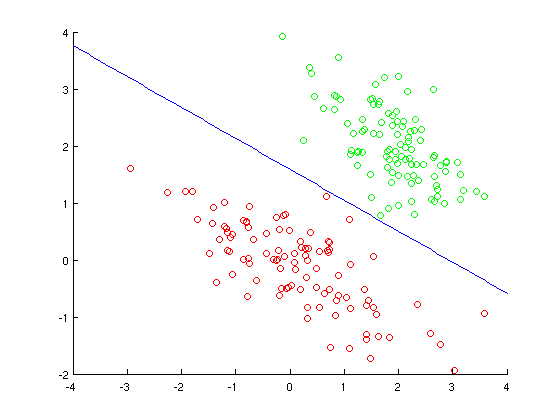
\includegraphics[scale = 0.5]{fig/perceptron_example.png}
\\
There is also another variant of the Perceptron algorithm, which is called Averaged Perceptron. They work in the same way, except that the Averaged Perceptron outputs the averaged weight vector instead of the final one.
\\\\
http://sites.stat.psu.edu/~jiali/course/stat597e/notes2/percept.pdf

\subsection{Text categorization}


\subsection{Programs and tools}
What tools and programs are already available for the problem, or for closely related ones?
Describe these briefly. Say how you can use them, and how your work will build on them, or differ from them. Explain which are relevant for your project and which not and why.
\\\\
* vilka program är vettiga att använda? -leta upp några-fördelar/nackdelar
skriv att vi valde matlab och varför.



